\documentclass[12pt,letterpaper]{article}
\usepackage[utf8]{inputenc}
\usepackage[english]{babel}
\usepackage{listings}
\usepackage{xcolor}
\usepackage{graphicx}

%For syntax highlighting
\definecolor{codegreen}{rgb}{0,0.6,0}
\definecolor{codegray}{rgb}{0.5,0.5,0.5}
\definecolor{codepurple}{rgb}{0.58,0,0.82}
\definecolor{backcolour}{rgb}{1,1,1}

%%Sets different parameters
\lstdefinestyle{mystyle}{
	backgroundcolor=\color{backcolour},   
    commentstyle=\color{codegreen},
    keywordstyle=\color{magenta},
    numberstyle=\tiny\color{codegray},
    stringstyle=\color{codepurple},
    basicstyle=\ttfamily\footnotesize,
    breakatwhitespace=false,         
    breaklines=true,                 
    captionpos=b,                    
    keepspaces=true,                 
    numbers=left,                    
    numbersep=5pt,                  
    showspaces=false,                
    showstringspaces=false,
    showtabs=false,                  
    tabsize=4
}
\lstset{style=mystyle}

\title{\textbf{Department of Computer Science and Engineering}}
\author{\textbf{S.G.Shivanirudh , 185001146, Semester VI }}

\date{4 February 2021}

\begin{document}
\maketitle
\hrule
\section*{\center{UCS1611 - Internet Programming Lab}}
\hrule 
\bigskip\bigskip

%Assignment name
\subsection*{\center{\textbf{Ex 01: Website for  International Conference using HTML5 Tags}}}

%Objective
\subsection*{\flushleft{Objective:}}
\begin{flushleft}
    Develop a Website for an International Conference using HTML5 elements. 
\end{flushleft}

%Code
\subsection*{\flushleft{Code:}}
\subsubsection*{\flushleft{Home Page:}}
\begin{flushleft}
\lstinputlisting[language = HTML]{index.html}
\end{flushleft}

\subsubsection*{\flushleft{Committee Page:}}
\begin{flushleft}
\lstinputlisting[language = HTML]{committee.html}
\end{flushleft}

\subsubsection*{\flushleft{Call For Papers Page:}}
\begin{flushleft}
\lstinputlisting[language = HTML]{paper.html}
\end{flushleft}

\subsubsection*{\flushleft{Important Dates Page:}}
\begin{flushleft}
\lstinputlisting[language = HTML]{dates.html}
\end{flushleft}

\subsubsection*{\flushleft{Workshops Page:}}
\begin{flushleft}
\lstinputlisting[language = HTML]{workshops.html}
\end{flushleft}

\subsubsection*{\flushleft{Registration Page:}}
\begin{flushleft}
\lstinputlisting[language = HTML]{registration.html}
\end{flushleft}

\subsubsection*{\flushleft{Contacts Page:}}
\begin{flushleft}
\lstinputlisting[language = HTML]{contact.html}
\end{flushleft}

\newpage
%Output
\subsection*{\flushleft{Output:}}
\subsubsection*{\flushleft{Home Page:}}
\begin{figure}[h]
    \centering
    
\includegraphics[width = \textwidth]{Pics/Home.png}
\end{figure}

\newpage
\subsubsection*{\flushleft{Committee Page:}}
\begin{figure}[h]
    \centering
    
\includegraphics[width = \textwidth]{Pics/Committee.png}
\end{figure}

\newpage
\subsubsection*{\flushleft{Call For Papers Page:}}
\begin{figure}[h]
    \centering
    
\includegraphics[width = \textwidth]{Pics/Papers.png}
\end{figure}

\newpage
\subsubsection*{\flushleft{Important Dates Page:}}
\begin{figure}[h]
    \centering
    
\includegraphics[width = \textwidth]{Pics/Dates.png}
\end{figure}

\newpage
\subsubsection*{\flushleft{Workshops Page:}}
\begin{figure}[h]
    \centering
    
\includegraphics[width = \textwidth]{Pics/Workshops.png}
\end{figure}

\newpage
\subsubsection*{\flushleft{Registration Page:}}
\begin{figure}[h]
    \centering
    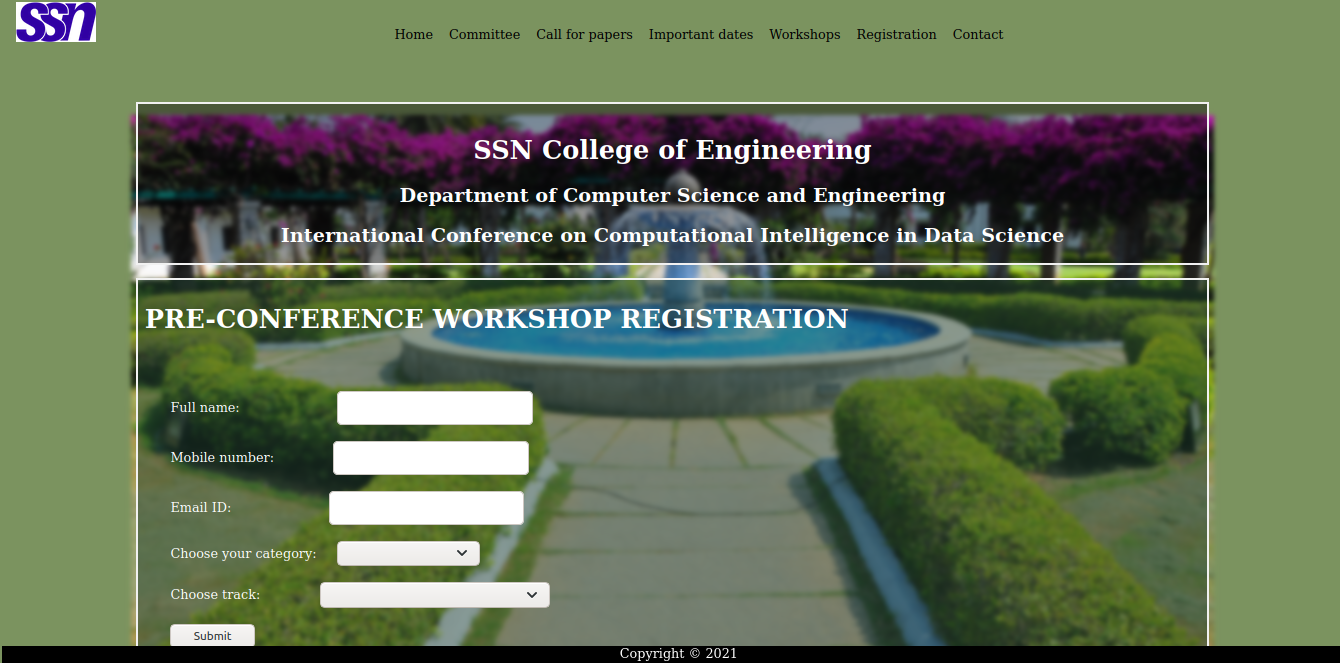
\includegraphics[width = \textwidth]{Pics/Registration.png}
\end{figure}

\newpage
\subsubsection*{\flushleft{Contacts Page:}}
\begin{figure}[h]
    \centering
    
\includegraphics[width = \textwidth]{Pics/Contact.png}
\end{figure}
\hrule

\subsection*{\flushleft{Learning Outcomes:}}
\renewcommand{\labelitemi}{$\textendash$}
\begin{itemize}
    \item Learnt to build a website with HTML5 only.
    \item Learnt to use inline styling by means of \textbf{style} attribute.
    \item Learnt the different types of tags in HTML5 and their varied uses.
\end{itemize}
\hrule
\end{document}